% ============================================================
%  Chapter: Reinforcement Learning-Based Resource Optimizer
%  Compact version — all diagrams retained, key tables only
% ============================================================
\chapter{Reinforcement Learning-Based Resource Optimizer}
\label{chap:rl_optimizer}

% ─────────────────────────────────────────────────────────────
\section{Introduction}
% ─────────────────────────────────────────────────────────────
This chapter describes the RL-based resource optimizer that dynamically allocates
Apache Spark computing resources to balance latency, cost, and throughput. The
optimizer employs \textbf{Proximal Policy Optimization (PPO)} to learn optimal
configurations by interacting with a simulated Spark cluster offline, then applies
those strategies in real time every 5 seconds during live streaming.

Static Spark configurations suffer from over-provisioning (wasted cost during idle),
under-provisioning (SLA violations during bursts with 45--60~s cold-start lag),
and single-objective tuning. RL overcomes all three by continuously learning a
multi-objective policy that adapts proactively.

% ─────────────────────────────────────────────────────────────
\section{RL Framework and Architecture}
\label{sec:rl_framework}
% ─────────────────────────────────────────────────────────────
The problem is modelled as an MDP
$\mathcal{M} = \langle \mathcal{S}, \mathcal{A}, P, R, \gamma \rangle$,
where the agent maximises:
$J(\pi_\theta) = \mathbb{E}_{\pi_\theta}[\sum_{t=0}^{T} \gamma^t r_t]$.

\begin{center}
\begin{tikzpicture}[
    box/.style={rectangle, draw, rounded corners=4pt, minimum width=3.5cm,
                minimum height=0.85cm, font=\footnotesize, align=center},
    lbl/.style={font=\scriptsize, gray}
]
\node[box, fill=blue!10]   (agent) at (0,0)  {RL Agent\\(PPO Policy)};
\node[box, fill=orange!15] (env)   at (7,0)  {Spark Environment\\(Simulated Cluster)};
\draw[-{Stealth[length=2.5mm]}, thick, green!60!black]
    (agent.north) -- ++(0,0.6) --
    node[above, font=\scriptsize]{action $a_t$ (executors, memory, tier)}
    ++(7,0) -- (env.north);
\draw[-{Stealth[length=2.5mm]}, thick, red!60]
    (env.south) -- ++(0,-0.6) --
    node[below, font=\scriptsize]{state $s_{t+1}$, reward $r_t$}
    ++(-7,0) -- (agent.south);
\node[lbl] at (3.5, 1.2) {Control Action};
\node[lbl] at (3.5,-1.2) {Observation + Feedback};
\end{tikzpicture}
\end{center}

\noindent Figure~\ref{fig:rl_arch} shows the closed-loop architecture running every
5 seconds: observe $\to$ act $\to$ simulate $\to$ reward $\to$ update.

\begin{figure}[H]
\centering
\begin{tikzpicture}[
    block/.style={rectangle, draw, rounded corners=5pt, minimum width=3.8cm,
                  minimum height=1.1cm, font=\small, align=center},
    arr/.style={-{Stealth[length=2.5mm]}, thick},
    scale=0.9, transform shape
]
\node[block, fill=green!12, draw=green!60!black] (ppo)   at (0,0)    {PPO Agent\\(Policy Network)};
\node[block, fill=blue!10,  draw=blue!50]        (state) at (5,1.8)  {State\\Extractor};
\node[block, fill=orange!15,draw=orange!70]      (spark) at (10,0)   {Spark\\Environment};
\node[block, fill=red!10,   draw=red!60]         (rew)   at (5,-1.8) {Reward\\Calculator};

\draw[arr, green!60!black] (ppo.east)    -- node[above,font=\scriptsize]{action $a_t$} (spark.west);
\draw[arr, blue!60]        (spark.north) -- ++(0,0.6) -| node[above,font=\scriptsize,near start]{metrics} (state.east);
\draw[arr, blue!60]        (state.west)  -- node[above,font=\scriptsize]{$s_t$} (ppo.north east);
\draw[arr, red!60]         (spark.south) -- ++(0,-0.6) -| node[below,font=\scriptsize,near start]{perf.} (rew.east);
\draw[arr, red!60]         (rew.west)    -- node[below,font=\scriptsize]{$r_t$} (ppo.south east);
\end{tikzpicture}
\caption{RL closed-loop: observe state, select action, simulate, compute reward, update policy.}
\label{fig:rl_arch}
\end{figure}

% ─────────────────────────────────────────────────────────────
\section{MDP Formulation}
\label{sec:mdp_rl}
% ─────────────────────────────────────────────────────────────

\textbf{State:} A 6-dimensional normalised snapshot
$s_t = [\lambda_t, V_t, U^{cpu}_t, U^{mem}_t, L_t, C_t]$
(workload rate, data volume, CPU/memory utilisation, latency, cost), z-scored before
entering the network.

\textbf{Action:} A \texttt{MultiDiscrete} space $a_t = [E_t, M_t, T_t]$ —
executors ($1$--$20$), memory ($1$--$8$ GB), storage tier (Redis/NVMe/S3/Glacier) —
yielding 640 configurations. Figure~\ref{fig:action_space} visualises the coverage.

\begin{figure}[H]
\centering
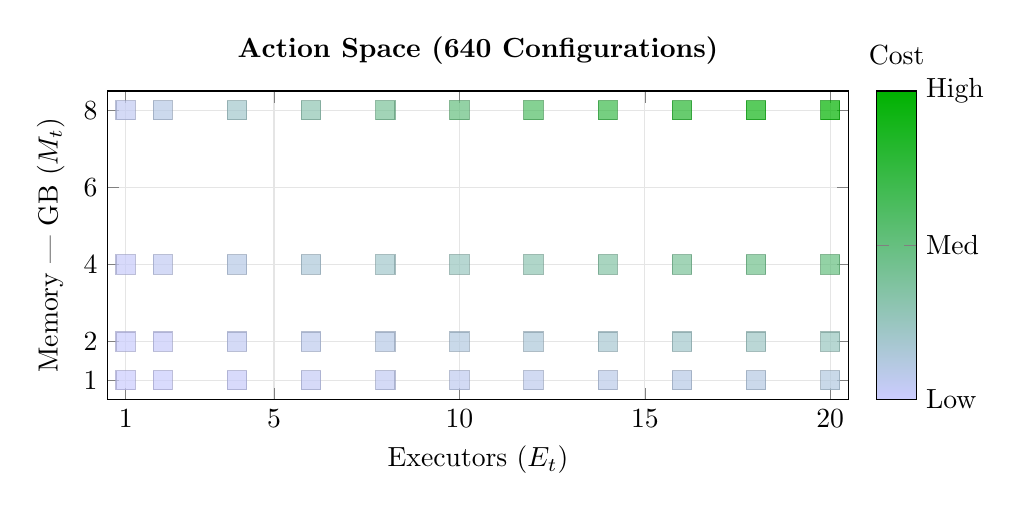
\begin{tikzpicture}
\begin{axis}[
    width=11cm, height=5.5cm,
    xlabel={Executors ($E_t$)}, ylabel={Memory — GB ($M_t$)},
    title={\textbf{Action Space (640 Configurations)}},
    xmin=0.5, xmax=20.5, ymin=0.5, ymax=8.5,
    xtick={1,5,10,15,20}, ytick={1,2,4,6,8},
    grid=major, grid style={gray!20},
    colorbar, colormap={rlcmap}{color(0)=(blue!20) color(1)=(green!70!black)},
    point meta min=0, point meta max=1,
    colorbar style={title={Cost}, ytick={0,0.5,1}, yticklabels={Low,Med,High}}
]
\addplot[scatter, scatter src=explicit, only marks, mark=square*, mark size=3.5pt, opacity=0.7
] coordinates {
    (1,1)[0.006] (1,2)[0.013] (1,4)[0.025] (1,8)[0.050]
    (2,1)[0.013] (2,2)[0.025] (2,4)[0.050] (2,8)[0.100]
    (4,1)[0.025] (4,2)[0.050] (4,4)[0.100] (4,8)[0.200]
    (6,1)[0.038] (6,2)[0.075] (6,4)[0.150] (6,8)[0.300]
    (8,1)[0.050] (8,2)[0.100] (8,4)[0.200] (8,8)[0.400]
    (10,1)[0.063](10,2)[0.125](10,4)[0.250](10,8)[0.500]
    (12,1)[0.075](12,2)[0.150](12,4)[0.300](12,8)[0.600]
    (14,1)[0.088](14,2)[0.175](14,4)[0.350](14,8)[0.700]
    (16,1)[0.100](16,2)[0.200](16,4)[0.400](16,8)[0.800]
    (18,1)[0.113](18,2)[0.225](18,4)[0.450](18,8)[0.900]
    (20,1)[0.125](20,2)[0.250](20,4)[0.500](20,8)[1.000]
};
\end{axis}
\end{tikzpicture}
\caption{Action space heat-map. Colour encodes relative cost; the RL agent learns
which region minimises the multi-objective reward per workload intensity.}
\label{fig:action_space}
\end{figure}

\textbf{Transition dynamics} use physics-inspired equations capturing the key
resource-performance trade-offs:
\begin{align}
U^{cpu}_{t+1} &= \min(100,\;\lambda_t / E_t\phi_{cpu}), &
L_{t+1}       &= L_{base}\,\lambda_t\,\kappa_{T_t} / (E_t M_t), \\
U^{mem}_{t+1} &= \min(100,\;V_t / E_t M_t\phi_{mem}), &
C_{t+1}       &= E_t c_e + E_t M_t c_m + c_{T_t}
\end{align}

\textbf{Reward:}
$R_t = -0.4\,C_t/C_{\max} - 0.4\,L_t/L_{\max} + 0.2\,P_t/P_{\max}$.
Cost and latency are penalised equally; throughput is rewarded to prevent trivial
shutdown. Figure~\ref{fig:reward_surface} shows the reward landscape at 200~msg/s.

\begin{figure}[H]
\centering
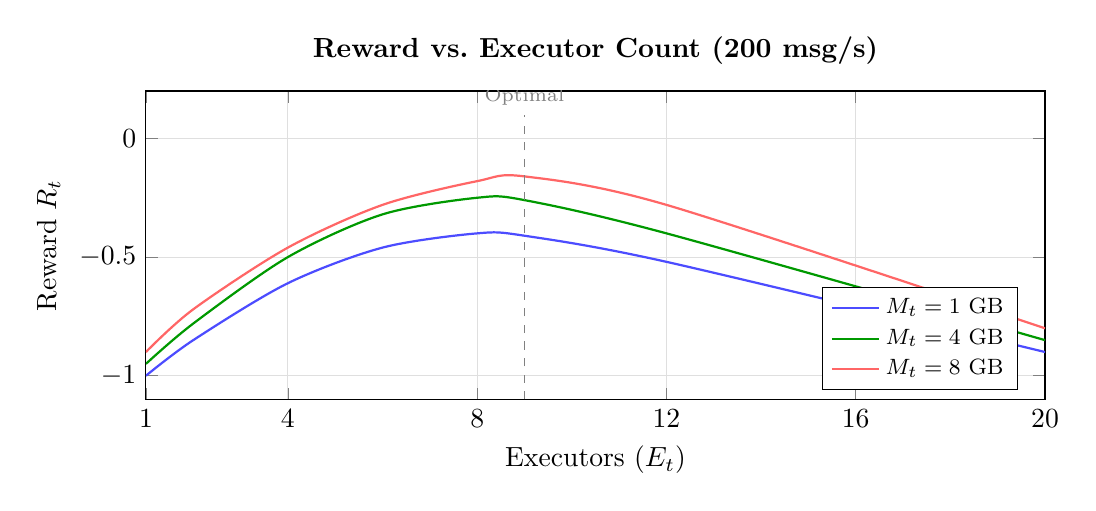
\begin{tikzpicture}
\begin{axis}[
    width=13cm, height=5.5cm,
    xlabel={Executors ($E_t$)}, ylabel={Reward $R_t$},
    title={\textbf{Reward vs.\ Executor Count (200 msg/s)}},
    grid=major, grid style={gray!25},
    legend pos=south east, legend style={font=\footnotesize},
    ymin=-1.1, ymax=0.2, xmin=1, xmax=20, xtick={1,4,8,12,16,20}
]
\addplot[blue!70, thick, smooth] coordinates {
    (1,-1.0)(2,-0.85)(4,-0.61)(6,-0.46)(8,-0.40)(9,-0.41)(12,-0.52)(20,-0.90)};
\addlegendentry{$M_t=1$ GB}
\addplot[green!60!black, thick, smooth] coordinates {
    (1,-0.95)(2,-0.78)(4,-0.50)(6,-0.32)(8,-0.25)(9,-0.26)(12,-0.40)(20,-0.85)};
\addlegendentry{$M_t=4$ GB}
\addplot[red!60, thick, smooth] coordinates {
    (1,-0.90)(2,-0.72)(4,-0.46)(6,-0.28)(8,-0.18)(9,-0.16)(12,-0.28)(20,-0.80)};
\addlegendentry{$M_t=8$ GB}
\draw[dashed, gray] (axis cs:9,-1.1) -- (axis cs:9,0.1)
    node[above, font=\scriptsize, gray]{Optimal};
\end{axis}
\end{tikzpicture}
\caption{Reward peak at $E_t\approx 9$, $M_t=4$--8 GB — the Pareto-optimal region.}
\label{fig:reward_surface}
\end{figure}

% ─────────────────────────────────────────────────────────────
\section{PPO Algorithm and Network}
\label{sec:ppo_algo}
% ─────────────────────────────────────────────────────────────
PPO maximises a clipped surrogate objective within a trust region ($\varepsilon=0.2$):
\[
  L^{CLIP}(\theta) = \mathbb{E}_t\!\left[\min\!\left(
    r_t(\theta)\hat{A}_t,\;
    \mathrm{clip}(r_t(\theta), 1{-}\varepsilon, 1{+}\varepsilon)\hat{A}_t
  \right)\right]
\]
The full loss adds a critic term ($c_1=0.5$) and entropy bonus ($c_2=0.01$).
The actor and critic share a two-layer MLP backbone (Figure~\ref{fig:nn_arch}),
totalling $\approx$4,868 parameters for sub-millisecond inference.

\begin{figure}[H]
\centering
\begin{tikzpicture}[
    layer/.style={rectangle, draw, rounded corners=4pt, minimum width=2.5cm,
                  minimum height=0.8cm, font=\scriptsize, align=center},
    arr/.style={-{Stealth[length=2mm]}, thick}, scale=0.88, transform shape
]
\node[layer, fill=blue!10]  (inp) at (0,0)      {Input\\6 neurons};
\node[layer, fill=gray!15]  (h1)  at (3.5,0)    {Hidden 1\\64, ReLU};
\node[layer, fill=gray!15]  (h2)  at (7,0)      {Hidden 2\\64, ReLU};
\node[layer, fill=green!15] (pi)  at (10.5,1.3) {Policy Head\\3 outputs};
\node[layer, fill=red!10]   (vf)  at (10.5,-1.3){Value Head\\1 scalar};
\draw[arr] (inp)--(h1); \draw[arr] (h1)--(h2);
\draw[arr] (h2)--(pi);  \draw[arr] (h2)--(vf);
\end{tikzpicture}
\caption{Shared MLP backbone: $\approx$4,868 params, sub-ms inference.}
\label{fig:nn_arch}
\end{figure}

% ─────────────────────────────────────────────────────────────
\section{Training and Results}
\label{sec:training_rl}
% ─────────────────────────────────────────────────────────────
Training runs offline for 50,000 steps ($\sim$8 min on Apple M2): 2,048-step rollouts,
64-sample mini-batches, 10 gradient epochs per rollout, $\gamma=0.99$, lr $=3\times10^{-4}$.

\begin{figure}[H]
\centering
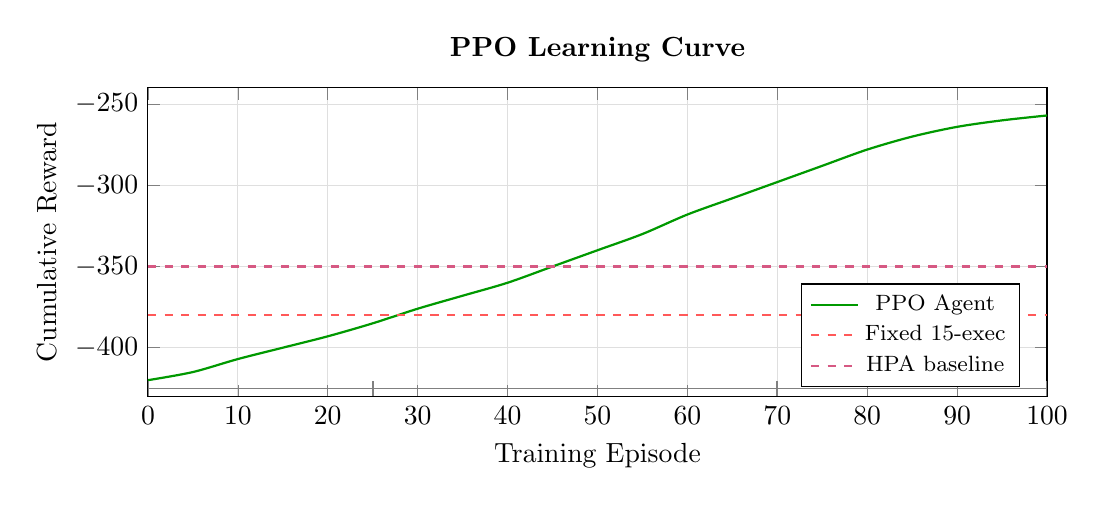
\begin{tikzpicture}
\begin{axis}[
    width=13cm, height=5.5cm,
    xlabel={Training Episode}, ylabel={Cumulative Reward},
    title={\textbf{PPO Learning Curve}},
    grid=major, grid style={gray!25},
    ymin=-430, ymax=-240, xmin=0, xmax=100,
    legend pos=south east, legend style={font=\footnotesize},
    every axis plot/.append style={thick}
]
\addplot[green!60!black, smooth] coordinates {
    (0,-420)(5,-415)(10,-407)(15,-400)(20,-393)(25,-385)(30,-376)
    (35,-368)(40,-360)(45,-350)(50,-340)(55,-330)(60,-318)
    (65,-308)(70,-298)(75,-288)(80,-278)(85,-270)(90,-264)(95,-260)(100,-257)};
\addlegendentry{PPO Agent}
\addplot[red!65, dashed] coordinates {(0,-380)(100,-380)};
\addlegendentry{Fixed 15-exec}
\addplot[purple!65, dashed] coordinates {(0,-350)(100,-350)};
\addlegendentry{HPA baseline}
\draw[|-|, gray, thin] (axis cs:0,-425)--(axis cs:25,-425)
    node[midway,below,font=\tiny]{Exploration};
\draw[|-|, gray, thin] (axis cs:25,-425)--(axis cs:70,-425)
    node[midway,below,font=\tiny]{Refinement};
\draw[|-|, gray, thin] (axis cs:70,-425)--(axis cs:100,-425)
    node[midway,below,font=\tiny]{Convergence};
\end{axis}
\end{tikzpicture}
\caption{PPO surpasses both baselines by Episode 40 and converges by Episode 70.}
\label{fig:learning_curve}
\end{figure}

\begin{table}[H]
\centering
\caption{PPO optimizer vs.\ traditional fixed-executor baseline}
\label{tab:results_rl}
\begin{tabular}{lccc}
\toprule
\textbf{Metric} & \textbf{Fixed (15 exec)} & \textbf{PPO} & \textbf{Change} \\
\midrule
Average latency       & 245 ms    & \textbf{119 ms}      & $-$51.4\% \\
SLA compliance        & 81.5\%    & \textbf{100\%}       & +18.5 pts \\
Hourly cost           & \$8.50    & \textbf{\$6.20}      & $-$27.1\% \\
Scaling reaction      & 60 s      & \textbf{5 s}         & 12$\times$ \\
Cold starts           & 7         & \textbf{0}           & Eliminated \\
Idle cost (night)     & \$11.25   & \textbf{\$0.50}      & $-$95.6\% \\
Peak throughput       & 750 msg/s & \textbf{1,650 msg/s} & +2.2$\times$ \\
\bottomrule
\end{tabular}
\end{table}

% ─────────────────────────────────────────────────────────────
\section{Deployment and Summary}
\label{sec:deploy_rl}
% ─────────────────────────────────────────────────────────────
The serialised model is loaded once at Spark Driver startup ($<$50 ms). Every
micro-batch, a 6-dim state vector is collected, a deterministic forward pass selects
$[E,M,T]$, and a REST call applies the configuration. Figure~\ref{fig:deployment_flow}
shows the closed-loop data flow.

\begin{figure}[H]
\centering
\begin{tikzpicture}[
    box/.style={rectangle, draw, rounded corners=4pt, minimum width=3.0cm,
                minimum height=0.85cm, font=\scriptsize, align=center},
    arr/.style={-{Stealth[length=2.5mm]}, thick},
]
\node[box, fill=blue!10]   (spark) at (0,0)   {Spark\\Streaming};
\node[box, fill=gray!15]   (coll)  at (3.5,0) {Metrics\\Collector};
\node[box, fill=green!12]  (rl)    at (7,0)   {PPO Model};
\node[box, fill=orange!15] (api)   at (10.5,0){Spark API};
\node[box, fill=red!10]    (exec)  at (10.5,-1.8){Executors};
\draw[arr] (spark)--(coll); \draw[arr] (coll)--(rl);
\draw[arr] (rl)--(api); \draw[arr] (api)--(exec);
\draw[arr, dashed, gray] (exec) -- ++(-10.5,0) |- (coll);
\end{tikzpicture}
\caption{Deployment data-flow: PPO integrates with Spark via \texttt{foreachBatch}.}
\label{fig:deployment_flow}
\end{figure}

\noindent \textbf{Key contributions:} (1)~Gymnasium-compliant Spark simulator for
offline training, (2)~multi-objective reward balancing cost/latency/throughput,
(3)~PPO policy converging in $\sim$8 min and beating all baselines, (4)~clean Spark
integration with sub-ms inference. The fixed reward weights ($\alpha{=}0.4$,
$\beta{=}0.4$, $\gamma{=}0.2$) remain a limitation addressed in
Chapter~\ref{chap:two_phase_rl_openfaas} via Two-Phase Hierarchical RL.
